\documentclass[sigconf]{acmart}

\settopmatter{printacmref=false} % Removes citation information below abstract
\renewcommand\footnotetextcopyrightpermission[1]{} % removes footnote with conference information in first column
\pagestyle{plain} % removes running headers

\usepackage{booktabs} % For formal tables
%\usepackage{hyperref}
\usepackage{listings}
\usepackage{color}

\definecolor{dkgreen}{rgb}{0,0.6,0}
\definecolor{gray}{rgb}{0.5,0.5,0.5}
\definecolor{mauve}{rgb}{0.58,0,0.82}

\lstset{frame=tb,
  language=Java,
  aboveskip=3mm,
  belowskip=3mm,
  showstringspaces=false,
  columns=flexible,
  basicstyle={\small\ttfamily},
  numbers=none,
  numberstyle=\tiny\color{gray},
  keywordstyle=\color{blue},
  commentstyle=\color{dkgreen},
  stringstyle=\color{mauve},
  breaklines=true,
  breakatwhitespace=true,
  tabsize=3
}


\setcopyright{none} % Copyright

\newcommand{\rpm}{\raisebox{.2ex}{$\scriptstyle\pm$}}

\begin{document}

\title{OSX System Measurement Project}

\author{Rebecca McKinley}
\affiliation{%
  \institution{University of California, San Diego}
}
\email{rmckinle@eng.ucsd.edu}

\author{Daniel Reznikov}
\affiliation{%
  \institution{University of California, San Diego}
}
\email{drezniko@eng.ucsd.edu}


\author{Aaron Trefler}
\affiliation{%
  \institution{University of California, San Diego}
}
\email{atrefler@eng.ucsd.edu}

%%%%%%%%%%%%%%%%%%%%%%%%%%%%%%%%%%%%%%%
% Abstract
%%%%%%%%%%%%%%%%%%%%%%%%%%%%%%%%%%%%%%%
\begin{abstract}
A characteristic challenge of profiling a computer system is the difficulty in isolating system components, accounting for control dependencies and optimizations, and conducting well-defined, repeatable experiments. The goal of this project is to profile an OSX Operation System and gain a more reasonable, big-picture understanding of how a personal computer's internal operations perform under certain conditions. We take measurements relating to the CPU, memory, network, and file system.
\end{abstract}

\maketitle

%%%%%%%%%%%%%%%%%%%%%%%%%%%%%%%%%%%%%%
% Introduction
%%%%%%%%%%%%%%%%%%%%%%%%%%%%%%%%%%%%%%
\section{Introduction}
In this project we measure the performance of our personal computer's components including its CPU, RAM, disk, and network capabilities. We implement the supporting measurement code primarily in C as it is familiar to us and is low-level enough to allow control of many system optimizations. All additional measurement code is implemented in x86 Assembly through the C interface. For certain measurements this gives us an even finer-grained control over the system's operations. We use GitHub as a mechanism for source control.

Our team members contribute equally to each part of the project. For each milestone, we walk through the design of each experiment together and implement equal parts individually. We have a regularly scheduled meeting time three days per week to ensure that most of the work is completed in a group setting. We have spent about 82 hours per person working on this project.

Section 2 describes the machine we use to take measurements as well as the steps we take to ensure a clean working environment. Section 3 measures and reports results for our system's CPU operations. Section 4 measures our system's memory operations. Section 5 discusses our network operations. Section 6 measures and reports our file system operations. Section 7 concludes.

For each section detailing our measurements (Sections 3 - 6), we have three subsections: \textit{Methodology} describes how our experiment is set up in detail, \textit{Results} shows a table or figure of our measurements and gives comments on our predicted and actual measurements as well as statistics, and \textit{Discussion} describes how we came to our prediction as well as what difficulties we encountered and if we believe our measurements were successful.

%%%%%%%%%%%%%%%%%%%%%%%%%%%%%%%%%%%%%%
% Machine Description
%%%%%%%%%%%%%%%%%%%%%%%%%%%%%%%%%%%%%%
\section{Machine Description}
\subsection{Machine Specifications}
Using the command \textit{sysctl hw} and the \textit{System Information} OSX utility, we are able to identify the characteristic metrics of each system component that impacts our performance profiling. The specification summary is detailed in Table \ref{spec}. We use \textit{gcc} on OSX which is linked to clang version 703.0.31.

\begin{table}[h!]
\centering
\caption{Local Machine Specification}
\label{spec}
\begin{tabular}{|l|l|}
\hline
\textbf{Component}	& \textbf{Specification}																										\\ \hline
CPU Model			& Intel Core i7, $2.7 GHz$, Dual Core																							\\ \hline
Cycle Time			& ($1/2.7GHz$) = $0.38ns$																										\\ \hline
L1 Cache			& \begin{tabular}[c]{@{}l@{}}Instruction Cache: $32KB$ (per core) \\ Data Cache: $32KB$ (per core)\end{tabular}					\\ \hline
L2 Cache			& $256KB$ (per core) Level 2 Cache																								\\ \hline
L3 Cache			& $6MB$ Total shared Level 3 Cache																								\\ \hline
RAM Size			& $16GB$ (2 Banks of $8GB$ DDR3)																								\\ \hline
Instruction Set		& x86-64																														\\ \hline
Memory Bus			& \begin{tabular}[c]{@{}l@{}}Type: DDR3\\ Speed: $1600MHz$\\ Width: 64-bit\end{tabular}											\\ \hline
I/O Bus				& \begin{tabular}[c]{@{}l@{}}Interconnect: SATA\\ Link Speed: 6 Gigabit\\ AHCI Version 1.30 Supported\end{tabular}				\\ \hline
Disk				& \begin{tabular}[c]{@{}l@{}}Capacity: $500GB$\\ Type: SSD\\ Mode: APPLE SSD SD512E\end{tabular}								\\ \hline
Network Card		& \begin{tabular}[c]{@{}l@{}}Card Type: AirPort Extreme (0x14E4, 0xEF)\\ Firmware Version: Broadcom BCM43xx 1.0\end{tabular}	\\ \hline
Operating System	& OSX 10.12																														\\ \hline
Compiler Version	& Clang v.703.0.31																							\\ \hline
\end{tabular}
\end{table}

\subsection{Setting Up Environment}
Due to the nature of most modern operating systems, there are several optimizations that we must turn off before we can take accurate measurements. This action comes with a consequence; the laptop we take measurements on will operate with temporarily reduced performance. Thankfully, it is possible to turn all of the optimizations back on once measurements are complete.

The first and most important consideration is our ability to turn off hyperthreading and the use of multiple cores. In the current OSX Macbook generation, it is possible to do this by entering the \textit{Instruments} application that comes as part of the Xcode developer tools. In \textit{Instruments} we can turn off hyperthreading and specify the number of cores to be used (only one) \cite{hyperthreading}.

The next important optimization removal is to disable TurboBoost. TurboBoost is a feature that comes with most modern OSX Macbooks and, when enabled, allows the processor to increase the clock speed on active cores \cite{shimpi_2011}. Keeping this on would make it extremely difficult to take accurate measurements with the \textit{rdtsc} register due to the inconsistent clock cycle time. To disable TurboBoost on OSX, we download a third party application called \textit{Turbo Boost Switcher} \cite{TurboBoostApp} that can enable and disable dynamic frequency scaling.

The last and simplest fix we implement to ensure accurate measurements was to use the \textit{nice} command that UNIX provides. By running \textit{nice -n --20 ./executable} we are able to request the highest priority for our program and ideally avoid the issue of context switching in the scheduler.

This is not a completely perfect system due to our lack of authority over exactly what the operating system might chose to do when we relinquish process control. However, we believe we account for the many optimizations in our system to the best of our abilities.

\subsection{Setting Up Experiments}
All of our experiments follow the setup given in the project description. For the purposes of this paper, we distinguish between iterations and experiments. An iteration is defined as one execution of the operation and one time measurement. One experiment encapsulates many iterations. The reported measurement for one experiment is calculated as the average time across all iterations in that experiment. Unless specified otherwise, all measurements reported in this paper use one million iterations and ten experiments with the final averages and standard deviations calculated across experiments.

%%%%%%%%%%%%%%%%%%%%%%%%%%%%%%%%%%%%%%%%%%%%%%%%%%%%%%%%%%%%%%%%%%%%%%%%%%%%
% CPU Operations
%%%%%%%%%%%%%%%%%%%%%%%%%%%%%%%%%%%%%%%%%%%%%%%%%%%%%%%%%%%%%%%%%%%%%%%%%%%%
\section{CPU Operations}

%%%%%%%%%%%%%%%%%%%%%%%% MEASUREMENT OVERHEAD %%%%%%%%%%%%%%%%%%%%%%%%%%%%%%%%%
\subsection{Measurement Overhead}
\subsubsection{Methodology}
The x86 Instruction Set Architecture (ISA) supports an operation that allows the processor to increment a special register value at every clock cycle. An \textit{rdtsc()} read will load a clock cycle count from the Time Stamp Counter (TSC). It has been shown \cite{isa} \cite{intelProfiling} that, in having an isolated environment optimization as described above, an \textit{rdtsc()} read can be implemented in x86 Assembly as follows \cite{bahra_2013}:

\begin{lstlisting}
static inline uint64_t rdtsc() {
  asm volatile("cpuid;" "rdtsc;" 
               : "+a" (eax), "=d" (edx) : 
               : "%rcx", "%rbx", "memory");
  asm volatile("xorl %%eax, %%eax;" "cpuid;" : : 
               : "%rax", "%rbx", "%rcx", "%rdx", "memory");
  return (((uint64_t)edx << 32) | eax);
}
\end{lstlisting}

To profile the overhead of reading time, we execute an experiment that makes two consecutive calls to \textit{rdtsc()}, computes the total number of elapsed cycles, and adds this to a running total that iterates this procedure several times. This method of reading the time via clock cycles works in tandem with the removal of OS optimizations as described in Section 1. Crucially, with only one core running our program, we can guarantee that the same \textit{rdtsc} register on the same CPU is queried each time. 

To profile the overhead of using a loop to measure many iterations of an operation, we orchestrate an experiment that executes an empty loop body, wrapping the loop in \textit{rdtsc()} calls.

\subsubsection{Results}
We aggregate many trials of this experiment. The summary of the predictions and the results are in Table \ref{MeasurementMetrics}.
 
\begin{table}[h!]
\centering
\caption{Metrics for Time Measurement and Loops}
\begin{tabular}{|l|l|l|}
\hline
\textbf{Metric}             & \textbf{rdtsc() ($ns$)}	& \textbf{Loop ($ns$)}	\\ \hline
Estimated Hardware Overhead & $7.40$ 		& $7.40$		\\ \hline
Estimated Software Overhead & $37.0$ 		& $18.5$		\\ \hline
Predicted Operating Time    & $44.4$ 		& $25.9$		\\ \hline
Measured Average Read Time  & $70.4$ 		& $11.4$		\\ \hline
Measured Std. Deviation 	& $0.25$		& $1.70$		\\ \hline
\end{tabular}
\label{MeasurementMetrics}
\end{table}

\subsubsection{Discussion}
The base hardware overhead is an estimate of how much time software is waiting on hardware. In both experiment scenarios, we execute fewer than a dozen assembly instructions and there is no I/O or network communication to stall the software. Because of these reasons, we expect the estimate for hardware overhead to be trivially small. For reading time, the user program executes the \textit{cpuid} instruction, does a bitwise \textit{xor} comparing register values, does a \textit{shift}, populates a return register, and terminates. We expect this to take about 20 cycles, or $8 ns$. For executing a loop, the hardware executes a \textit{bne} (branch not equal) instruction, an empty loop body, and a \textit{jump}. From these estimations, we expect the hardware overhead for loops and reading to be comparable.

The software overhead for reading time is limited to the work that needs to be done to move the running code into memory, and to jump from the executing experiment body to the \textit{rdtsc()} definition. We expect that the software overhead for running the loop body is also trivially small.

Our predictions for both experiments are on the same order as the measured results. We are pleased to find that the experiments have little variance across trials, which increases our confidence that the methods appropriately isolate the measurement overhead functionality that we are interested in profiling.

%%%%%%%%%%%%%%%%%%%%%%%% PROCEDURE CALL OVERHEAD %%%%%%%%%%%%%%%%%%%%%%%%
\subsection{Procedure Call Overhead}
\subsubsection{Methodology} 
In this section we report the incremental overhead of an argument to a procedure call. We do this by measuring the procedure call overhead for eight different procedures that take zero to seven integer arguments. The procedures are implemented as functions in C with only a return statement as their function body. To measure the overhead for a procedure call, we perform ten experiments that call the procedure one million times per experiment. We then average the results over these experiments to calculate our final overhead for the procedure calls.

\subsubsection{Results}
The estimated results for the procedure call overhead experiments can be found in Table \ref{ProcedureCallOverheadEstimated} and the measured results can be found in Table \ref{ProcedureCallOverheadActual}.

\begin{table}[h!]
\centering
\caption{Estimated Metrics for Procedure Calls}
\label{ProcedureCallOverheadEstimated}
\begin{tabular}{|l|l|l|l|}
\hline
\textbf{No. Args} & \multicolumn{1}{c|}{\begin{tabular}[c]{@{}c@{}}\textbf{Estimated} \\ \textbf{Hardware} \\\textbf{Overhead ($ns$)}\end{tabular}} & \begin{tabular}[c]{@{}l@{}}\textbf{Estimated}\\ \textbf{Software} \\\textbf{Overhead ($ns$)}\end{tabular} & \multicolumn{1}{c|}{\begin{tabular}[c]{@{}c@{}}\textbf{Predicted} \\ \textbf{Operating} \\\textbf{Time ($ns$)}\end{tabular}} \\ \hline
$0$ & $13.0$ & $37.0$ & $50.0$ \\ \hline
$1$ & $13.3$ & $37.0$ & $50.4$ \\ \hline
$2$ & $13.7$ & $37.0$ & $50.7$ \\ \hline
$3$ & $14.1$ & $37.0$ & $51.1$ \\ \hline
$4$ & $14.4$ & $37.0$ & $51.5$ \\ \hline
$5$ & $14.8$ & $37.0$ & $51.9$ \\ \hline
$6$ & $15.2$ & $37.0$ & $52.2$ \\ \hline
$7$ & $15.6$ & $37.0$ & $52.6$ \\ \hline
\end{tabular}
\end{table}

\begin{table}[h!]
\centering
\caption{Measured Metrics for Procedure Calls}
\label{ProcedureCallOverheadActual}
\begin{tabular}{|l|l|l|}	
\hline
\textbf{No. Args} & \multicolumn{1}{c|}{\begin{tabular}[c]{@{}c@{}}\textbf{Measured Average} \\ \textbf{Operating Time  ($ns$)}\end{tabular}} & \multicolumn{1}{c|}{\begin{tabular}[c]{@{}c@{}}\textbf{Measured Std.} \\\textbf{Deviation  ($ns$)}\end{tabular}} \\ \hline
$0$ & $51.1$ 	& $17.0$ \\ \hline
$1$ & $52.6$	& $17.4$ \\ \hline
$2$ & $51.9$	& $16.7$ \\ \hline
$3$ & $52.2$	& $16.7$ \\ \hline
$4$ & $52.2$	& $16.7$ \\ \hline
$5$ & $51.5$	& $16.3$ \\ \hline
$6$ & $52.2$	& $16.3$ \\ \hline
$7$ & $53.3$	& $16.7$ \\ \hline
\end{tabular}
\end{table}

\subsubsection{Discussion} 
We hypothesize that we will see an increase in procedure call overhead as the number of arguments increases because it will require the system hardware to store more values in its registers during a procedure call. Thus, we estimate that the software overhead will be consistent for each procedure call, but the hardware overhead will increase by a single cycle for each argument added. See Table \ref{ProcedureCallOverheadEstimated} for our estimates prior to running the experiment.

In order for a procedure call to execute, the caller must place the first six integer arguments into registers. Any parameters beyond six will need to be redirected and placed in other areas of the memory hierarchy. After the call is executed, the call instruction pushes the return address to the stack. Before the function body executes, it adjusts the stack pointer as needed. The procedure then executes its code. Before the return happens, the function needs to clean up after itself by rewinding the stack back to its state after the function call. After the return, the return address is popped off the stack and placed into the program counter. After cleanup, the caller pops any parameters off the stack so that it is returned to its initial state \cite{nico}. This process informed both our hardware and software estimates.

Our results confirm our hypothesis that we would see an increase in procedure call overhead as the number of arguments increased. Fitting a least-squares regression line between the \textit{Number of Arguments} and \textit{Procedure Call Cycles}, we see that for each argument added, the the number of cycles increases by approximately $1.3$ cycles. See Figure \ref{ProcedureCallRegPlot} for analysis details.

It also worth pointing out that we see a significant jump in procedure call execution time between six and seven arguments, which supports our earlier claim that any parameters beyond six will need to be redirected.

\begin{figure}[h]
\caption{Procedure Arguments vs. Overhead Time}
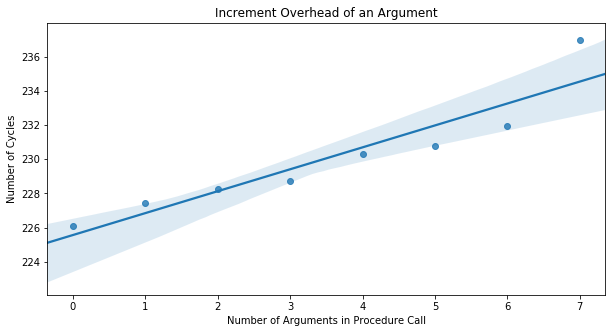
\includegraphics[scale=0.40]{images/procedure_call_overhead_regplot.png}
\label{ProcedureCallRegPlot}
\end{figure}

%%%%%%%%%%%%%%%%%%%%%%%% SYSTEM CALL OVERHEAD %%%%%%%%%%%%%%%%%%%%%%%%
\subsection{System Call Overhead}
\subsubsection{Methodology}
In this section we measure the overhead for executing a system call. The most important aspect of this measurement is that we avoid caching in its operation. If a process caches the return value, it will not give an honest measurement of the trap to the kernel. To avoid this, we execute each system call in a separate forked process. 

We use the \textit{getPid()} system call due to its simple structure and (ideally) low processing overhead as compared to other system operations. In our implementation, the child process of a \textit{fork()} polls for the time, calls \textit{getPid()}, then polls again for the time. The nature of forked processes allows us to avoid the caching issue because each call to \textit{getPid()} was that process' first time accessing its pid. Additionally, each forked child has a unique pid. In this way, we are able to circumvent any caching operation. We did put some effort into running the trap routine ourselves through asm inline assembly code in C, but were unable to successfully implement it.

\subsubsection{Results}
\begin{table}[h!]
\centering
\caption{Metrics for a System Call}
\begin{tabular}{|l|l|}
\hline
\textbf{Metric}             	& \textbf{Time ($\mu s$)} 	\\ \hline
Estimated Hardware Overhead 	& $0.0555$					\\ \hline
Estimated Software Overhead 	& $0.556$					\\ \hline
Predicted Operating Time    	& $0.611$					\\ \hline
Measured Average Operating Time	& $90.5$					\\ \hline
Measured Std. Deviation 		& $26.7$					\\ \hline
\end{tabular}
\label{SysCallMetrics}
\end{table}
The performance estimations and measurements for a system call are given in Table \ref{SysCallMetrics}.

\subsubsection{Discussion}
During a typical system call, the hardware must execute an interrupt service routine in order to trap to the kernel. This requires calling the \textit{int 0x80} instruction to indicate to hardware that a system call is needed \cite{gupta_2014}. The base hardware should not take many cycles to execute a minimal system call because in \textit{getPid()} the only hardware operation required is to load the \textit{syscall} value located in the register, identify and return the value to software, and read and return the value of the current process' pid. For hardware alone this would require in the order of tens of cycles to complete and should not yield significant overhead.

The software overhead in a system call is much more significant due to the operations of the kernel. A system call does not call the trap directly, instead it is an interface into a library call that will check that the user has the necessary permissions and validate the parameters. This is where caching can come into play. The software starts the trap and waits for the hardware. At this point the privileges have been elevated and kernel code can now execute using kernel privileges. The kernel requests a read of the current process id and returns it back to the user. Software overhead is significantly higher than hardware overhead in the case of a system call. We would expect the software to do the heavy lifting.

The results we measured did not completely align with our expectations. Our measured operating time was significantly higher than our estimated cycles. We expect this is due to our inability to control exactly where the operating system will enter after calling \textit{getPid()}. Another potential issue could be in our baseline hardware and software estimates. We are confident that our understanding of a system call's operation is accurate, but we have underestimated how long it actually takes. We find that the cost of a system call is much greater than that of a procedure call. This is expected because of the additional software and hardware overhead needed to execute a trap and the time allocated to allow the operating system to execute.

%%%%%%%%%%%%%%%%%%%%%%%% TASK CREATION OVERHEAD %%%%%%%%%%%%%%%%%%%%%%%%
\subsection{Task Creation Overhead}
\subsubsection{Methodology}
For the purposes of this project there are two definitions of a task: one as a separate process, and another as a kernel thread. We use \textit{fork()} to spawn a new process and \textit{pthread\_create()} from the \textit{pthread.h} library to generate kernel threads.

For process creation, we construct a pipe for communication between the parent and child process. The parent starts by taking a time measurement, calling \textit{fork()}, and waiting on their child. The child process takes the ending time measurement as its first operation. The child then sends the recorded time to its parent through the pipe and exits. The parent receives the end time and subtracts the start and end value to get the elapsed time to create a process. This time is further reduced by the read overhead time. We run many iterations of this code, average the creation time, and repeat these iterations for multiple trials.

For thread creation, we start by taking the beginning time measurement. We then call \textit{pthread\_create()} to spawn a new thread. The executing thread function takes the time as its first operation. The spawned thread then returns the recorded time. Meanwhile, the originating thread does a \textit{join} and waits on the spawned thread to conclude execution. It records the returned value and subtracts it from the start time in order to calculate the time to execute a pthread creation. We also subtract the overhead for reading time. Similar to process creation, we run many iterations of this code, average the creation time, and repeat these iterations for multiple trials.

\subsubsection{Results}
\begin{table}[h!]
\centering
\caption{Metrics for Process and Thread Creation}
\begin{tabular}{|l|l|l|}
\hline
\textbf{Metric}					& \textbf{Process ($\mu s$)}	& \textbf{Thread ($\mu s$)}	\\ \hline
Estimated Hardware Overhead		& $0.556$						& $0.278$					\\ \hline
Estimated Software Overhead		& $278$							& $5.56$					\\ \hline
Predicted Operating Time		& $278$							& $5.83$					\\ \hline
Measured Average Operating Time	& $732$							& $22.8$					\\ \hline
Measured Std. Deviation			& $975$ 						& $1.32$					\\ \hline
\end{tabular}
\label{ProcThreadCreationMetrics}
\end{table}
The performance and estimations for the creation of a process and a thread is located in Table \ref{ProcThreadCreationMetrics}.

\subsubsection{Discussion}
When a new process is created the operating system must create and copy a completely new page table for the child, copy all relevant data including the stack and registers, allocate a new address space, update the program counter, and many more operations \cite{cs4411}. The operating system software manages the majority of these operations and needs to update its internal software management structures. As such, the amount of cycles spent in hardware and software is highly dependent on what the current state of the parent process is at the time of creation. We estimate a low hardware cycle count ($0.556 \mu s$) as compared to the software cycle count ($278 \mu s$). The numbers are based on the cycles recorded in the previous section relating to a system call.

By comparison, creating a thread is a much less intensive operation than creating a process. In thread creation, we expect that the majority of time is spent on the software side in order to create a lightweight process. When a new thread is generated, the operating system must allocate new registers and a new stack. This is significantly less than the overhead of creating a processes. Threads share the same address space and can refer to shared data segments without penalty from the hardware or software \cite{robbins_2000}. However, the creation of a thread does mean that the operating system needs to do more management. Shared data makes accesses more complex and requires additional verification checks.

The time to create a process was much higher than we had predicted. Because creating a process is such a complicated task, we cannot entirely predict how much needs to be done in order to generate all the data and space for a new process. We likely did not account for the additional overhead in operating system management that must oversee this execution. The estimations are based on our measurements for system calls. However, it seems there are more complex calls in \textit{fork()} and it involves more intensive work than we initially anticipated.

The time to create a kernel thread was higher than we had predicted. However, we were much closer in our estimation with threads than we were with our estimation of processes. This is most likely because we had initially underestimated the time to create a process and then based our estimation for a thread off of the underestimated process. We expect that the pthread library must do additional operations in thread creation. And it most likely provides some assistance to the operating system during creation.

The relationship between process creation time and thread creation time was as we expected. Creating a process takes almost 32 times as long as creating a thread. This is due to the fact that an entirely new process requires more overhead up front to allocate and distribute the additional resources. Kernel threads share enough resources between them that the overhead for creation only should rightfully be considered less. In this aspect we would consider our measurements to be a success as they logically make sense.

%%%%%%%%%%%%%%%%%%%%%%%% CONTEXT SWITCH OVERHEAD %%%%%%%%%%%%%%%%%%%%%%%%
\subsection{Context Switch Overhead}
\subsubsection{Methodology}
The \textit{pipe()} function exposes two desirable utilities to this experiment. First, it enables our system to force a process/thread to wait for another process/thread. And second, it facilitates the sharing of data, specifically the results of timing calls to \textit{rdtsc()}. We utilize the pipe blocking semantics to force a context switch to the responding process.

To measure the time of a context switching between processes, our code creates a new process with \textit{fork()}. Both the parent and child measure time with \textit{rdtsc()} and the child writes its time measurement to the pipe and exits. Depending on whether the child or parent process runs first, the code measures the context switch from child to parent or parent to child. The blocking pipe semantics are crucial for the experiment; they ensure that we do not rely on a specific ordering of process execution. If the parent is first to execute, they will read from an empty pipe, causing a block. Once blocked, the OS will trigger a context switch to the child who will take a time measurement and write to the pipe. Once exited, the parent is unblocked and they can read the time from the pipe. If the child executes first, then the child will take a timing measurement and write to the empty pipe before exiting. This triggers a context switch to the parent who will read the time value from the pipe without issue. In both cases, a single context switch can be measured.

To measure the time of a context switch between two threads of the same process, we launch a new thread with \textit{pthread\_create()}, linking them semantically with a \textit{pipe()}, and joining them logically with a call to \textit{pthread\_join}. Both threads measure time and the absolute difference gives the time for a context switch. The justification is similar to that of a context switch between processes.

\subsubsection{Results}
Each trial creates a process or thread, forces a context switch, and computes the time. The results are compiled in Table \ref{ContextSwitchOverhead}.

\begin{table}[h!]
\centering
\caption{Context Switch Overhead}
\begin{tabular}{|l|l|l|}
\hline
\textbf{Metric}             & \textbf{Process ($\mu s$)}	& \textbf{Thread ($\mu s$)}	\\ \hline
Estimated Hardware Overhead & $185$							& $92.6$					\\ \hline
Estimated Software Overhead & $37.0$						& $37.0$					\\ \hline
Predicted Operating Time    & $222$							& $130$						\\ \hline
Measured Average Time     	& $313$							& $14.1$					\\ \hline
Measured Std. Deviation 	& $0.032$						& $0.002$					\\ \hline
\end{tabular}
\label{ContextSwitchOverhead}
\end{table}

\subsubsection{Discussion}
A process context switch requires the state of the current running process to be saved to a PCB (Process Control Block) data structure. A handle to the saved PCB is stored in order to load the process back when it gets scheduled. The scheduler runs to select another process, the TLB is flushed, and the next process PCB is loaded, and the process resumes execution right where it left off. 

The hardware overhead is spread between flushing the PCB and executing two memory I/O requests for loading/retrieving the PCB. We estimate this to be on the order of $500K$ cycles $(185 \mu s)$. Assuming the PCB preparation is software managed, the software overhead may be on the order of an additional $100K$ cycles $(37 \mu s)$, estimating the time for a process context switch to be roughly $600K$ cycles $(222 \mu s)$.

For a context switch between threads, much of the same series of operations need to happen, except that a TLB flush is not necessary because threads share the same virtual memory. We estimate the hardware overhead to be half of that of a process, $250K$ cycles $(93 \mu s)$, and the software overhead to be comparable at $100K$ cycles $(37 \mu s)$. The estimate for the total time to context switch between threads is on the order of $350$ cycles $(130 \mu s)$.

Our estimate for the process context switch is reasonably close, but we underestimate the benefit savings of avoiding TLB flushes during thread context switches. The results show that threads switch an order of magnitude faster than processes, implying that much more time than we had originally suspected is spent in the hardware during this procedure.

%%%%%%%%%%%%%%%%%%%%%%%%%%%%%%%%%%%%%%%%%%%%%%%%%%%%%%%%%%%%%%%%%%%%%%%%%%%%
% Memory Operations
%%%%%%%%%%%%%%%%%%%%%%%%%%%%%%%%%%%%%%%%%%%%%%%%%%%%%%%%%%%%%%%%%%%%%%%%%%%%
\section{Memory Operations}

%%%%%%%%%%%%%%%%%%%%%%%% RAM ACCESS TIME %%%%%%%%%%%%%%%%%%%%%%%%%%%%%%%%%
\subsection{RAM Access Time}
The Mac Operating System has three levels of CPU cache lines that the OS uses in exploiting spatial and temporal locality for memory accesses. As described in Table \ref{spec}, these cache lines correspond to per core sizes of $32KB$ (L1), $256KB$ (L2), and $6MB$ (L3), where L3 is shared across all cores. This section outlines profiling of integer accesses to each of these memory regions - that is, the average latency of loading a 4-byte value from each of these regions.

\subsubsection{Methodology}
In closely following the methodology described in the lmbench paper we measure the "back-to-back load" which, "is the time that each load takes, assuming that the instructions before and after are also cache missing loads" \cite{lmbench}. This level of granularity is readily implemented in software.

We prepare arrays of pointers of varying sizes between $1KB$ and $512MB$. We consider iterations to be the number of accesses during an experiment where each access is an integer load. A goal for this measurement was to avoid prefetching. Prefetching happens when the operating system utilizes spacial locality to preemptively load a cache line it believes the user will need next. It is a useful optimization when iterating through an array or any other fixed-stride operation. However we want to avoid this optimization in our measurement because it would speed up access time. The architecture calculates the line to fetch by calculating the previous stride. However modern architectures are not good at calculating pointer stride. In order to avoid prefetching, we stride over an array of pointers with varying stride sizes between $2$ and $2^{20}$ in incremental powers of two. The pointer array allows us to load a stored pointer (a 4-byte value) during each update as follows:

\begin{lstlisting}
for (int i = 0; i < iterations; i++) {
	idx = (ptr + stride) % array_size
	ptr = array[idx]
}
\end{lstlisting}

We wrap this loop in calls to \textit{rdtsc()}, normalize the cycle count by iterations, and average it over many experiments for statistical convergence. Each stride size loads integers from each array size defined in order to span each region of memory.

\subsubsection{Results}
\begin{figure}[h!]
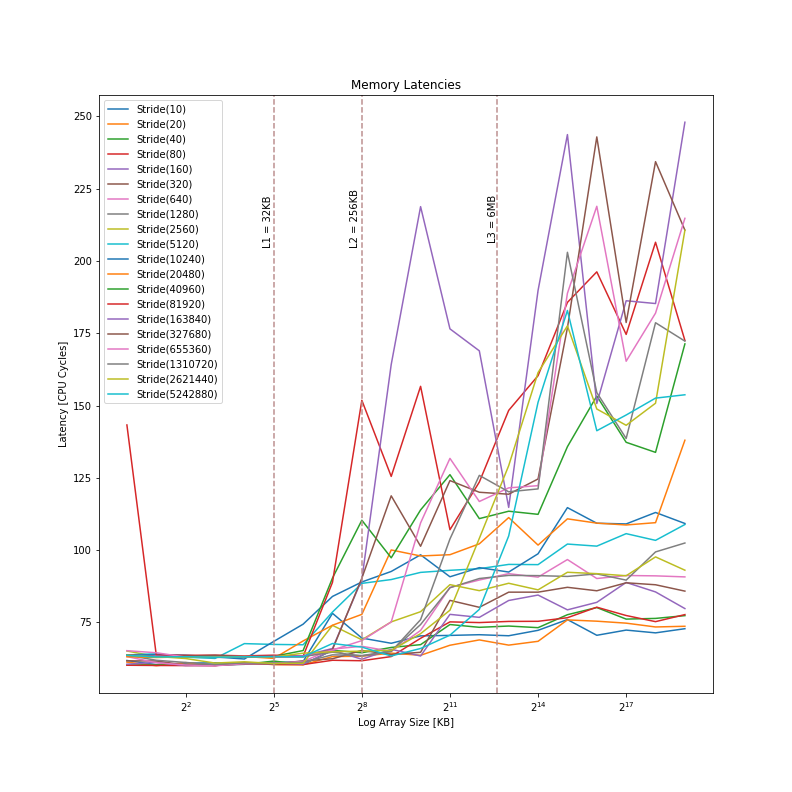
\includegraphics[scale=0.33]{images/Memory_Latencies.png}
\caption{Log-Scale File Access vs. Time}
\label{memoryLatency}
\end{figure}
Our experimental results are shown in Figure \ref{memoryLatency}.

\subsubsection{Discussion}
The results in Figure \ref{memoryLatency} make us confident in our measurements because of the spikes near each change in memory region. Specifically, we observe access times of $30$, $60$, $100$, and $300$ CPU cycles for L1, L2, L3, and RAM respectively. At $2.7GHz$, this corresponds to $11$, $22$, $37$ and $111ns$, respectively.

These results are commensurate with our expectations. The latency to each subsequent cache level is roughly double and the RAM latency is some orders of magnitude higher than the L1 cache. These results are consistent with nominal specifications of comparable architectures.

Despite our confidence in our measurements, we did expect each region to plateau more when causing hits in their respective caches. We expected this because the access time is a function of the memory region and should not vary much with the precise amount of data read from that particular region. We surmise that the plateaus would be more evident if we had taken array sizes to have a finer granularity.

%%%%%%%%%%%%%%%%%%%%%%%% RAM BANDWIDTH %%%%%%%%%%%%%%%%%%%%%%%%%%%%%%%%%
\subsection{RAM Bandwidth}
In modern operating systems there are several optimizations that can make bandwidth benchmarking difficult. The most significant of which is the caching and prefetching mechanisms that are designed to speed up memory accesses. In normal operations, this is a benefit and an optimization. However, for bandwidth measurements we want to focus on main memory and not the caches. We take two strategies to avoid caching and prefetching, one for reading and one for writing, as described below.

\subsubsection{Methodology}
For writing bandwidth, we use the Intel SSE intrinsics to avoid cache lines. Intel intrinsics are C-style functions that are an abstraction above x86 assembly; they provide simple access to low level operations \cite{Intel_Intrins}. A class of store intrinsics allows for non-temporal memory accesses. Non-temporal instructions indicate to the OS that this data will not be used again soon, so there is no need to cache it \cite{drepper_2007}. This allows us to perform writes that will always fetch data in main memory and not store it in the cache. We start by allocating an array of values larger than the L3 cache size and setting some initial values. This allows us to avoid any storage into the cache and to ensure that all pages are loaded into main memory. We also unroll to the loop by a factor of eight due to the fact that an integer is four bytes long and we have 64-bit cache lines. From there, we run several experiments with multiple iterations of storing values into the allocated array.

For reading bandwidth we take a somewhat different approach. We could not find non-temporal load intrinsics, so we decide to use the strategy of unrolling and adding as specified in the lmbench paper \cite{Brown:1997:OSB:258623.258690}. We again start by allocating large arrays that would not fit into the L3 cache and then copy data from one array to another. We unroll the loop as detailed above and perform a memory access and an addition operation. In order to avoid the data access being optimized, we store the values into a counter that is marked as a volatile register. This allows us to ensure that the compiler will not optimize the values away.

\subsubsection{Results}
\begin{table}[h!]
\centering
\caption{Measured RAM Bandwidth}
\begin{tabular}{|l|l|l|}
\hline
\textbf{Metric}				& \textbf{Reading $(GB/s)$}	& \textbf{Writing $(GB/s)$}	\\ \hline
Predicted Operating Time	& $25.6$					& $25.6$					\\ \hline
Measured Average Time		& $10.0$					& $15.0$					\\ \hline
Measured Std. Deviation		& $1.11$					& $0.267$					\\ \hline
\end{tabular}
\label{RAMBandwidth}
\end{table}
The results can be seen in Table \ref{RAMBandwidth}. We give our predicted operating time as calculated in the next section along with the averages and standard deviations for reading and writing.

\subsubsection{Discussion}
In order to find our estimates, we look to our machine specifications in Table \ref{spec}. Our machine's memory operates at $1600MHz$ with 2 banks of 64-bit DDR3. We can derive the equation \((1,600,000,000 \text{ } clock\text{ }cycles / second)*(2\text{ }lines / clock)*(64\text{ }bits / line) = 204,800,000,000\text{ }bits / second\). Corresponding to \(25.6GB/s\). This is listed in Table \ref{RAMBandwidth} as our predicted operating time. It is difficult to extract the exact hardware and software overhead in terms of a bandwidth; however we consider all data transfer to be done on the hardware memory bus and the software overhead to be less involved due to the lack of copying needed.

Even though our ideal calculations are sound, it is highly unlikely that it is our true peak bandwidth. Most likely this measurement is one that is only possible in the most ideal of circumstances and is not possible to replicate perfectly. Even after accounting for the manufacturer's idealism, our measurements are close to the ideal reading. We believe our methodology is successful in avoiding speed-up from cache hits or slow-down from disk accesses. Low variance increases our confidence. 

It is interesting to note that the measured bandwidth for reading was lower than that for writing. Some deviation is to be expected because of the inconsistent implementation between reading and writing bandwidth. We would normally expect the writing bandwidth to be lower since there are more operations to be done with a write. We believe this is due to the fact that with the writing bandwidth measurement we were able to use the SSE intrinsics. With intrinsics, we have a much better understanding and an increased guarantee of what the system is doing in its operation. As predicted, we consider our writing measurements to be a more accurate representation of the system than our reading measurements.

%%%%%%%%%%%%%%%%%%%%%%%% PAGE FAULT SERVICE TIME %%%%%%%%%%%%%%%%%%%%%%%%%%%%%
\subsection{Page Fault Service Time}
For this section we report the time taken for faulting an entire page from disk. 

\subsubsection{Methodology}
We force a page fault by ensuring data is mapped to the virtual address space of a program, while ensuring it is not mapped to any physical memory location. We then read a byte of data from this virtually mapped data to incur the desired page fault. The specific details of methodology are as follows:

\begin{enumerate}
	\item Clean the memory cache of the system using the \textit{purge} system call. 
	\item Map $3GB$ of data to a program's virtual address space using the \textit{mmap()} system call.
	\item Read a byte from the virtual address space created in the previous step.
	\item Derive the page fault time as the time needed to read the byte, less the time for loop overhead and two \textit{rdtsc()} calls.
\end{enumerate}

This process was repeated ten times in order to produce our final results.

\subsubsection{Results}
The results we obtained from our experiment are listed in Table \ref{PageFaultResults}.

\begin{table}[!ht]
\centering
\caption{Page Fault Service Time}
\begin{tabular}{|l|l|l|}
\hline
\textbf{Metric}             	& \textbf{Time ($ms$)}	\\ \hline
Estimated Hardware Overhead 	& $0.180$				\\ \hline
Estimated Software Overhead 	& $0.240$				\\ \hline
Predicted Operating Time    	& $0.420$				\\ \hline
Measured Average Time     		& $0.220$				\\ \hline
Measured Std. Deviation 		& $0.030$				\\ \hline
\end{tabular}
\label{PageFaultResults}
\end{table}

\subsubsection{Discussion}
A major page fault requires internal OS computations involving procedure calls (e.g., determining the page is not currently in physical memory), data transfer via the I/O and memory buses, and disk accesses in order to retrieve the desired page. The hardware overhead is primarily concerned with disk read and transfer times. For our SSD, the average sequential read speed is $21.3MB/s$ \cite{ssdrating} and we are reading one page of memory, which is $4KB$. As such, we expect the hardware overhead to contribute $0.18 ms$ to the overall runtime. We expect the software overhead to take a much more significant portion of the runtime. We believe software computations will take $0.32ms$ (i.e., approximately five procedure calls as measured by our previous experiment). Thus, the total predicted time for a page fault on our system came to $0.42ms$.

Our measured page fault time was faster than our predicted page fault time, though both were on the same order of magnitude (i.e., tenths of milliseconds). The standard deviation was an order of magnitude less than the average. Because of this we feel confident in the experiment results reported.

We compare the measured page fault time to the amount of time it would take to access a block of data on RAM. Our system has an ideal RAM bandwidth of $25.6GB/s$, which corresponds to $0.16ms$ per $4KB$ block. Thus, we would estimate that accessing a block of data from RAM on our system is approximately $27\%$ faster than accessing it from disk.

%%%%%%%%%%%%%%%%%%%%%%%%%%%%%%%%%%%%%%
% Network
%%%%%%%%%%%%%%%%%%%%%%%%%%%%%%%%%%%%%%
\section{Network Operations}
All measurements for network operations are done in Python version 2.7.10. We decided to use Python because it simplified the network setup time. For measurements on the network, we did not need the fine-grained control that C provides. This was also recommended to us by the professor. We use a different method for calculating time, but because the measurements are coarse-grained and will execute in the millisecond granularity, we do not lose any accuracy.

All local measurements are taken on the local machine described at the beginning of this report in Table \ref{spec}. For the remote measurements, we chose a machine that was very similar to our local one in order to have the most consistent measurements. The specifications for our remote machine are located in Table \ref{RemoteMachineSpec}. For all experiments, the local machine was the client and the remote machine executed the server.

\begin{table}[h!]
\centering
\caption{Remote Machine Specification}
\label{RemoteMachineSpec}
\begin{tabular}{|l|l|}
\hline
\textbf{Component}	& \textbf{Specification}																										\\ \hline
CPU Model			& Intel Core i7, $2.5 GHz$, Dual Core																							\\ \hline
Cycle Time			& ($1/2.5GHz$) = $0.4ns$																										\\ \hline
L1 Cache			& \begin{tabular}[c]{@{}l@{}}Instruction Cache: $32KB$ (per core) \\ Data Cache: $32KB$ (per core)\end{tabular}					\\ \hline
L2 Cache			& $256KB$ (per core) Level 2 Cache																								\\ \hline
L3 Cache			& $6MB$ Total shared Level 3 Cache																								\\ \hline
RAM Size			& $16GB$ (2 Banks of $8GB$ DDR3)																								\\ \hline
Instruction Set		& x86-64																														\\ \hline
Memory Bus			& \begin{tabular}[c]{@{}l@{}}Type: DDR3\\ Speed: $1600MHz$\\ Width: 64-bit\end{tabular}											\\ \hline
I/O Bus				& \begin{tabular}[c]{@{}l@{}}Interconnect: SATA\\ Link Speed: 6 Gigabit\\ AHCI Version 1.30 Supported\end{tabular}				\\ \hline
Disk				& \begin{tabular}[c]{@{}l@{}}Capacity: $500GB$\\ Type: SSD\\ Mode: APPLE SSD SD512E\end{tabular}								\\ \hline
Network Card		& \begin{tabular}[c]{@{}l@{}}Card Type: AirPort Extreme (0x14E4, 0xEF)\\ Firmware Version: Broadcom BCM43xx 1.0\end{tabular}	\\ \hline
Operating System	& OSX 10.13.4																													\\ \hline
\end{tabular}
\end{table}

%%%%%%%%%%%%%%%%%%%%%%%% ROUND TRIP TIME %%%%%%%%%%%%%%%%%%%%%%%%%%%%%
\subsection{Round Trip Time}
\subsubsection{Methodology}
The experiment for measuring round trip time (RTT) is taken using both a server and a client. The server opens and binds a socket for listening on the network, while the client connects to that socket. The client constructs a 64-byte packet of data to send over to the server. We choose 64 bytes because it matches the size of the packet a \textit{ping} sends over the network. The client starts a timer and sends the packet to the server using \textit{sendall()}. The server blocks on its \textit{recv()} until it has received the full data from the client before it echoes the received packet back to the client. Once the client receives the full data back, it ends its timer and reports statistics.

For the local measurement, the IP address is \textit{127.0.0.1}. For the remote host, the two computers connect on a mobile hotspot network. This avoids some issues of network contention. The IP address is found by running the \textit{ifconfig} command on the remote server machine.

The ping measurements were taken in much the same way, simply by running \textit{ping IP-ADDRESS}.

\subsubsection{Results}
\begin{table}[h!]
\centering
\caption{Local RTT Measurements}
\label{LocalRTTMeasurements}
\begin{tabular}{|l|l|}
\hline
\textbf{Metric}								& \textbf{Overhead $(ms)$}	\\ \hline
Estimated Local Hardware Overhead			& $1.0 e{-5}$				\\ \hline
Estimated Local Software Overhead			& $2.69 e{-5}$				\\ \hline
Predicted Local Operating Time				& $3.69 e{-5}$				\\ \hline
Measured Average Local \textit{ping} Time	& $0.189$					\\ \hline
Measured Average Local Operating Time		& $0.179$					\\ \hline
Measured Std. Deviation						& $0.015$					\\ \hline
\end{tabular}
\end{table}

\begin{table}[h!]
\centering
\caption{Remote RTT Measurements}
\label{RemoteRTTMeasurements}
\begin{tabular}{|l|l|}
\hline
{\textbf{Metric}}							& {\textbf{Overhead ($ms$)}}	\\ \hline
Estimated Remote Hardware Overhead			& $1.00$						\\ \hline
Estimated Remote Software Overhead			& $2.00$						\\ \hline
Predicted Remote Operating Time				& $3.00$						\\ \hline
Measured Average Remote \textit{ping} Time	& $47.9$						\\ \hline
Measured Average Remote Operating Time		& $7.11$						\\ \hline
Measured Std. Deviation						& $0.993$						\\ \hline
\end{tabular}
\end{table}
The local results for this experiment, including the local ping time, are in Table \ref{LocalRTTMeasurements}. The remote results for this experiment are in Table \ref{RemoteRTTMeasurements}.

\subsubsection{Discussion}
For local operations, we do not expect there to be much or any hardware overhead. The loopback interface is a special interface that specifies a virtual network for local communication and we do not expect this virtual interface to have much in terms of hardware operation \cite{Loopback}. The software overhead will be more significant. The kernel will need to copy the data to and from the buffers for sending and receiving as well as streaming data. We predict that a send involves a write while a receive involves both a read and a write. In total between the server and the client, we expect there to be four write operations and two read operations on 64 bytes of data each. Using the RAM bandwidth measurements as a rough heuristic ($10GB/s$ for reading and $15GB/s$ for writing), we calculate an estimated $0.0269 \mu s$ as our software overhead.

Our estimation was smaller than our measured results. However, we are very confident in our measured value because our experiment is sound and it matches the results from the \textit{ping} command closely. The \textit{ping} took slightly longer than our local measurements, which surprised us, but it is not a significant difference. We attempted to normalize the ping cycles, but some iterations did take longer or shorter depending on the state of the machine. In general we would expect a \textit{ping} to execute faster because it operates at a kernel level and does not need to trap. Additionally, it is an optimized library that is more closely coupled with the operating system.

For remote operations, we expect there to be more hardware overhead. In fact, we see a significant difference in the measured operating time between local and remote execution. This is expected because contention for the remote network is high; there are many users attempting to use this network and we are limited by the throughput of our connection. Even with our privatized wireless system, there is contention in how the mobile hotspot itself connects to its network. In the case of hardware overhead, the network card has to do more work to make the connection and send packets. The software overhead is also expected to be more significant because the packets need to go through validation, streaming, and routing.

Similar to the local experiment, our predictions were too conservative. Our remote operating time was many times higher than our local measurements, but they are within the same logical units of $ms$. We feel confident in our measured remote values partially because we felt confident in our local values. The code is sound and we set up the connection correctly. However, for remote execution, our measurement differs significantly from the remote \textit{ping}. This is surprising to us especially since the ping for local execution was so close to our measured value. The main justification we can see for why the \textit{ping} is higher is that there is more overhead for networking and security in a ping. Our code implicitly trusts the connected server and does not have a long handshake process. Additionally, the data our code transmits is only received and never processed.

%%%%%%%%%%%%%%%%%%%%%%%% PEAK BANDWIDTH %%%%%%%%%%%%%%%%%%%%%%%%%%%%%
\subsection{Peak Bandwidth}
\subsubsection{Methodology}
To measure the network bandwidth, we want to transmit the largest packet possible to measure the data transfer rate. The connection code is similar to that done for measuring RTT: the server creates a socket and binds it to a port while the client creates a socket to connects to the server. The client then creates a very large packet of data; $300MB$ worth. We chose this size through a combination of execution time and the measurements in the lmbench paper \cite{lmbench}. Once the server receives an initial acknowledgement, it starts the timer and blocks on \textit{recv()} until it receives all $300MB$ of data from the client. Once all data is received, the server records the end time and statistics in units of $MB/s$.

\subsubsection{Results}
\begin{table}[h!]
\centering
\caption{Measured Local and Remote Bandwidth}
\label{LocalRemoteBandwidthMeasurements}
\begin{tabular}{|l|l|l|}
\hline
\textbf{Metric}						& \textbf{Local ($MB/s$)}	& \textbf{Remote ($MB/s$)}	\\ \hline
Predicted Operating Time			& $366$						& $9.00$					\\ \hline
Measured Average Operating Time		& $640$						& $24.9$					\\ \hline
Measured Std. Deviation				& $0.25$					& $1.24$					\\ \hline
\end{tabular}
\end{table}
The results of both the local and remote network bandwidth measurements are shown in Table \ref{LocalRemoteBandwidthMeasurements}.

\subsubsection{Discussion}
For the TCP protocol, the maximum window size is $2^{16} bytes$, or $64KB$ \cite{greer_2018}. There exists a window scaling factor that can increase the length of this up to $256KB$. We expect this window size to be the limiting factor in our bandwidth calculations. We measured our local RTT as $0.179ms$, so we expect the local bandwidth to be in the range of $366 MB/s$. We calculate our remote prediction in a similar way.

We consider both our local and remote bandwidth measurements to be a success. One reason for the difference in measurement could be that our TCP protocol is not using the maximum TCP window size or it is utilizing the window scaling factor. It is surprising to us how different the local and remote bandwidths are. We expect the remote bandwidth to be much lower, but not necessarily that much lower. This is a result of the network having enough traffic to cause contention with our program, and the fact that many systems on our machines need to access the network. The processing time on both machines is significant in the case of remote execution due to network overhead.

For both our bandwidth and RTT measurements we do not feel that we achieved close to the ideal hardware performance for several reasons. The most important of these being the bottleneck in the LTE network. There is a limit to the bandwidth of our network connection. Another issue could be in network hardware contention. The performance measurements for these pieces of hardware are taken in the most ideal of circumstances - with little interference and a lot of external bandwidth available. However in our use case, there are several programs other than the our benchmarking running and contending for resources. Another reason we might not be achieving peak hardware performance is because we are using a wireless connection. A physically wired Ethernet connection would be a better scenario to measure hardware performance because it reduces the number of potential bottlenecks in the system. It would be an interesting extension to this experiment to wire both computers together with a physical cable and take these measurements.

%%%%%%%%%%%%%%%%%%%%%%%% CONNECTION OVERHEAD %%%%%%%%%%%%%%%%%%%%%%%%%%%%%
\subsection{Connection Overhead}
\subsubsection{Methodology}
This final network experiment utilizes the same setup and tear-down code that the previous measurements used. For this experiment we isolate this code and do no network transfer operations. The server code starts by creating a socket with \textit{socket.socket()} and doing a \textit{bind()} on port $59030$. Then the server sets to \textit{listen()} for an incoming connection. On the client's end, they start similarly by creating a socket with \textit{socket.socket()} before calling \textit{connect()} to make an initial connection to the server. At this point the time is recorded - this measures setup time. The client then starts up another timer before calling \textit{socket.shutdown()} and \textit{socket.close()} to simulate a tear-down operation. The end time is recorded and statistics are reported for tear-down.

\subsubsection{Results}
\begin{table}[h!]
\centering
\caption{Measured Local Setup and Tear-Down Time}
\label{LocalSetupTearDownMeasurement}
\begin{tabular}{|l|l|l|}
\hline
\textbf{Metric}					& \textbf{Setup ($ms$)}	& \textbf{Tear-Down ($ms$)}	\\ \hline
Est. Local Hardware Overhead	& $0.050$				& $0.025$					\\ \hline
Est. Local Software Overhead	& $0.100$				& $0.050$					\\ \hline
Predicted Local Operating Time	& $0.150$				& $0.075$					\\ \hline
Meas. Avg. Local Operating Time	& $0.260$				& $0.0581$					\\ \hline
Meas. Std. Deviation			& $0.013$				& $0.0081$					\\ \hline
\end{tabular}
\end{table}

\begin{table}[h!]
\centering
\caption{Measured Remote Setup and Tear-Down Time}
\label{RemoteSetupTearDownMeasurement}
\begin{tabular}{|l|l|l|}
\hline
\textbf{Metric}						& \textbf{Setup ($ms$)}	& \textbf{Tear-Down ($ms$)}	\\ \hline
Est. Remote Hardware Overhead		& $0.100$				& $0.050$					\\ \hline
Est. Remote Software Overhead		& $0.200$				& $0.100$					\\ \hline
Predicted Remote Operating Time		& $0.300$				& $0.150$					\\ \hline
Meas. Avg. Remote Operating Time	& $9.50$				& $0.245$					\\ \hline
Meas. Std. Deviation				& $0.232$				& $0.0344$					\\ \hline
\end{tabular}
\end{table}
The results for local setup and tear-down time are located in Table \ref{LocalSetupTearDownMeasurement}. The results for remote setup and tear-down time are located in Table \ref{RemoteSetupTearDownMeasurement}.

\subsubsection{Discussion}
For setup time, a TCP connection requires a three step handshake protocol between communicating parties: SYN, SYN-ACK, and ACK. From these three messages we expect a local hardware setup time of $0.05ms$ based on our measured local RTT and $0.10ms$ for remote hardware setup time based on our remote RTT. Software overhead for a setup operation includes validating sequence numbers, validating packets, copying data, and simply waiting. Because of this, we expect the software overhead to similarly correspond to the RTT software overhead.

For tear-down time, the TCP connection requires a four-way handshake with FIN, ACK, FIN, ACK. There is less waiting during tear-down since it comes in the middle of communication and the second ACK is sent immediately from the receiving procedure. We predict that the tear-down would be around half of the setup time.

We consider our methodology to be a success. We have very similar results to our predicted outcomes. It is also as expected that the setup takes much longer than tear-down. The extent to which the remote setup time differed from the local setup time was surprising. However, due to the similar remote/local measurement relationship established in the previous section, it is makes sense. It is also worth noting that the setup and tear-down time is comparable to the RTT times. This indicates to us that when sending a packet the initial setup and tear-down contribute significantly the total running time.

%%%%%%%%%%%%%%%%%%%%%%%%%%%%%%%%%%%%%%
% File System
%%%%%%%%%%%%%%%%%%%%%%%%%%%%%%%%%%%%%%
\section{File System}
The file system is a crucial consideration in the design of an operating system. OSX uses Apple's proprietary Apple File System (APFS) which has sophisticated mechanisms for recovery, protection, and performance. We aim to experimentally measure basic performance of I/O bound workloads on APFS, including the file buffer cache, local and remote read times for sequential and random disk accesses, and how process contention for disk access impacts read time.

%%%%%%%%%%%%%%%%%%%%%%%% FILE CACHE SIZE %%%%%%%%%%%%%%%%%%%%%%%%%%%%%
\subsection{Size of the File Cache}
OSX will dynamically allocate a sizable portion of main memory to a file buffer cache, This will cache needed disk pages to reduce the overhead of disk bound I/O. This experiment measures the precise size of the file buffer cache. 

\subsubsection{Methodology}
First, we generate a $16GB$ file of random data. An experiment corresponds to different file read sizes ranging from $8MB$ to $16GB$. Each experiment iteration reads its given number of bytes from the file in order to load it into the file buffer cache. The experiment then purges (flushes) the cache lines with the \textit{purge()} system call. Then we again read the given number of bytes from the file pointer using the \textit{fread()} API, wrapping it in calls to \textit{rdtsc()} to measure time. 

We read the file backwards in order to limit the ability of the processor to optimize page prefetching. As an example, if we are executing an experiment with $1GB$, we would read the last $1GB$ of the file for the first iteration. Experiments are done while no other applications are running on the system to limit RAM contention.

\subsubsection{Results}
\begin{figure}[h!]
\caption{Average I/O Latency per Block Read}
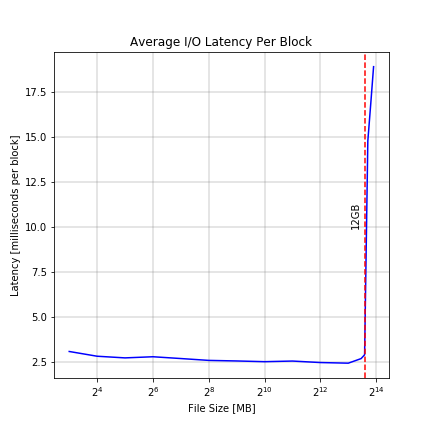
\includegraphics[scale=0.60]{images/fileCacheSizeResults.png}
\label{fileBufferCacheLatency}
\end{figure}
The results in Figure \ref{fileBufferCacheLatency} show the read time latency as a function of the size of the file being read. The x-axis shows the file size being read and the y-axis shows the average latency measured. The measured I/O time is normalized by the number of blocks read for easy comparison.

\subsubsection{Discussion}
The file I/O latency increases dramatically when reading $12GB$ files. This indicates to us that the file buffer cache size is approximately $12GB$. Using the built-in OSX Activity Monitor, we can see that the system has approximately $2.5GB$ of wired memory and $1GB$ of compressed memory. This leaves almost $14GB$ of memory for the OS to use. Since the system was under minimal load during experimentation, it makes sense that almost the entirety of this available memory bank is given to the file buffer cache during the I/O intensive measurements.

We note two complications in reading this data. First, the time measured encapsulates both memory access time in addition to the time to \textit{memcopy()} data into the process address space. We do not have a good way of subtracting this cost. When the data is in the file buffer cache, this may be a sizable operation. However, it is a common operation for each experiment which allows for integrity of relative measurements. When the block needs to be paged in from disk, the cost of the \textit{memcopy()} operation is insignificant in comparison.

The second issue to note is that the data is presented as measured time, normalized by blocks read. This means we are not accurately presenting the real latency because a large part of the file may still be cached. For example, $12GB$ out of a $13GB$ file may be in the file buffer cache. The latency for reading $13GB$ is disproportionately large compared to the latency of reading a file that fits entirely into the file cache. But the y-value of this data point in Figure \ref{fileBufferCacheLatency} has been averaged over total blocks read, which includes blocks that were in the file cache. This average pulls the data point down, implying that the latency of the disk I/O may be two orders of magnitude higher than the cache latency, not one order of magnitude as might be read from the plot.

These points do not detract from the goal of this experiment. We are confident that our setup has identified the precise size that a file buffer cache can reach on the system, namely $12GB$.

%%%%%%%%%%%%%%%%%%%%%%%% FILE READ TIME %%%%%%%%%%%%%%%%%%%%%%%%%%%%%
\subsection{File Read Time}
In this section we report both the sequential and random access character reading times on our system as a function of file size.

\subsubsection{Methodology}
For each experiment we: 
\begin{enumerate}
\item Create several files of random data of the following sizes: $32KB$, $64KB$, $128KB$, $256KB$. We perform all the following steps for each of these file sizes.
\item Perform sequential access by reading a character from each page of the file starting from the first character, and utilizing the \textit{fseek()} command to advance the file access pointer forward by our page-size, $4KB$, between each read command.
\item Perform random access by reading a character from each page of the file, and utilizing \textit{fseek()} to  move the file access pointer to the beginning of a random page within the file between each read command.
\end{enumerate}

We measure the time taken for all character reads during the experiment. We run ten experiments in order to produce our results.

Additionally, we ensure that we were not measuring cached data by (1) turning off data caching using the \textit{fcntl} command with the \textit{"F NOCACHE"} flag and (2) running \textit{purge}, which forces the disk cache to be flushed and emptied prior to every character read.

\subsubsection{Results}
Results for our experiment are listed in Table \ref{SequentialFileReadTimes} and Table \ref{RandomFileReadTimes}, as well as shown in Figure \ref{FileReadTimePlot}.

\begin{table}[h!]
\centering
\caption{Sequential Access File Read Times}
\label{SequentialFileReadTimes}
\begin{tabular}{|l|l|l|l|l|}
\hline
\textbf{Metric ($\mu s$)}	& \textbf{32KB}	& \textbf{64KB}	& \textbf{128KB}  & \textbf{256KB}  \\ \hline
Predicted Time				& $72$			& $61$			& $56$			& $53$				\\ \hline
Meas. Avg. Time				& $143$			& $108$			& $96$			& $85$				\\ \hline
Meas. Std. Dev.				& $67$			& $27$			& $29$			& $24$				\\ \hline
\end{tabular}
\end{table}

\begin{table}[h!]
\centering
\caption{Random Access File Read Times}
\label{RandomFileReadTimes}
\begin{tabular}{|l|l|l|l|l|}
\hline
\textbf{Metric ($\mu s$)}	& \textbf{32KB} & \textbf{64KB}	& \textbf{128KB}	& \textbf{256KB}	\\ \hline
Predicted Time				& $72$			& $61$			& $56$				& $53$				\\ \hline
Meas. Avg. Time				& $87$			& $93$			& $91$				& $81$				\\ \hline
Meas. Std. Dev.				& $19$			& $20$			& $27$				& $23$				\\ \hline
\end{tabular}
\end{table}

\begin{figure}[h]
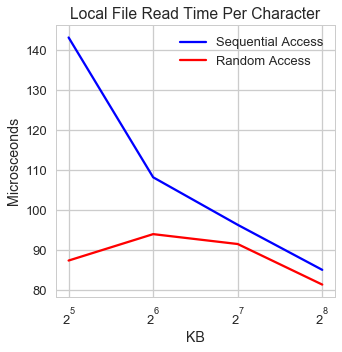
\includegraphics[scale=0.7]{images/file_read_time.png}
\caption{Log-Log Size of File vs. Avg Block Access Time}
\label{FileReadTimePlot}
\end{figure}

\subsubsection{Discussion}
Prior to making our predictions for this section, we wish to highlight the following points:

\begin{enumerate}
	\item When the first character of the file is read, it will incur a page fault.
	\item Due to the initial page fault, our system will respond by bringing in the complete contents of the file being accessed into RAM. This is because our largest file for this experiment, $256KB$, can easily fit into our system's memory.
	\item Since our system uses an SSD for non-volatile storage, randomly accessing the contents of a file will not be any slower or faster than accessing the file's contents sequentially.
\end{enumerate}

Therefore, we predict the average time taken to read a character from a block of a file to be:

$$\frac{\text{page fault time} + (\text{n\_blocks} - 1)\ \cdot\ \text{memory access time}} {\text{n\_blocks in file}}$$
  
We estimate \textit{"page fault time"} to be $220\mu s$. We estimate \textit{"memory access time"} to be $50.4\mu s$. We derive our estimate for \textit{"memory access time"} by predicting that it will take $0.4\mu s$ to move the data from RAM and an additional $50 \mu s$ for overhead. This overhead accounts for such things as: sending the request to RAM, locating the memory requested, and slowdown due to competition with other processes also attempting to access memory. We predict the same file read times for both sequential and random access. Our predictions take into account both our general knowledge as well as preliminary results from previous sections of our report (i.e., RAM Bandwidth and Page Fault Service Time).

As hypothesized, we do not see a significant difference between the file read times between sequential and random access experiments.

Our predicted times were slightly lower than our measured times, though they were within a reasonable amount of error given the standard deviations. We hypothesize that the lower predicted times were due to us underestimating the "memory access time" incurred upon each read after the initial page fault.

The project description asks us to discuss the sense in which our sequential access might not be "sequential". When a program requests many data blocks sequentially from a file, the operating system goes to the file's inode and loads the necessary data blocks. Those data blocks might not be sequential on disk due to fragmentation. Even when we believe we are accessing a set of block sequentially, they may not be arranged on disk sequentially.

%%%%%%%%%%%%%%%%%%%%%%%% REMOTE FILE READ TIME %%%%%%%%%%%%%%%%%%%%%%%%%%%%%
\subsection{Remote File Read Time}
In this section we report both the sequential and random access remote character reading time as a function of file size.

\subsubsection{Methodology}
For this section we re-run the experiment utilized in the previous section on File Read Time, but ensured file access was performed over a network. We accomplish this by storing and accessing files on a second machine. The second machine has specifications almost identical to our system and is described in Table \ref{RemoteMachineSpec}. The network utilized was a 4G LTE hotspot setup by an Iphone 8.

\subsubsection{Results}
Results for our experiment are listed in Table \ref{RemoteSequentialFileReadTimes} and Table \ref{RemoteRandomFileReadTimes}, as well as shown in Figure \ref{RemoteFileReadTimePlot}.

\begin{table}[h!]
\caption{Remote Sequential Access File Read Times}
\label{RemoteSequentialFileReadTimes}
\begin{tabular}{|l|l|l|l|l|}
\hline
\textbf{Metric ($\mu s$)}	& \textbf{32KB}	& \textbf{64KB}	& \textbf{128KB} & \textbf{256KB} 	\\ \hline
Predicted  					& $2,062$		& $1,456$		& $1,153$		& $1,001$			\\ \hline
Meas. Avg.					& $39,145$		& $27,172$		& $6,675$		& $4,537$			\\ \hline
Meas. Std. Dev. 			& $33,097$		& $11,036$		& $4,369$		& $3,329$			\\ \hline
\end{tabular}
\end{table}

\begin{table}[h!]
\caption{Remote Random Access File Read Times}
\label{RemoteRandomFileReadTimes}
\begin{tabular}{|l|l|l|l|l|}
\hline
\textbf{Metric ($\mu s$)}	& \textbf{32KB} & \textbf{64KB} & \textbf{128KB}	& \textbf{256KB}   	\\ \hline
Predicted Time				& $2,062$		& $1,456$		& $1,153$			& $1,001$			\\ \hline
Meas. Avg. Time				& $29,555$		& $7,584$		& $8,263$			& $3,982$			\\ \hline
Meas. Std. Dev.				& $21,715$		& $22,857$		& $4,651$			& $1,939$			\\ \hline
\end{tabular}
\end{table}

\begin{figure}[h]
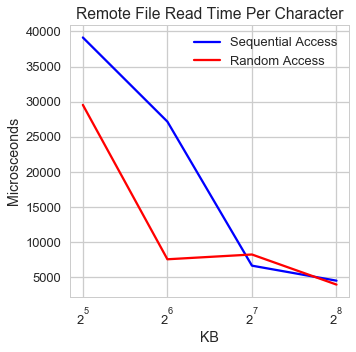
\includegraphics[scale=0.7]{images/remote_file_read_time.png}
\caption{Log/log plot with the x-axis the size of the file and y-axis the average per-block time.}
\label{RemoteFileReadTimePlot}
\end{figure}

\subsubsection{Discussion}
In order to make our prediction for remote file read times, we wish to highlight the following points:

\begin{enumerate}
	\item When the first character of the file is read remotely, the system will send over all the contents of the file from the remote machine and save it into its local RAM. This is because the largest file for this experiment is $256KB$, which can easily fit into our system's memory.
	\item Since the remote system uses an SSD for non-volatile storage, randomly accessing the contents of a file will not be any slower or faster than accessing the file's contents sequentially.
\end{enumerate}

Therefore, we predict the average time taken to read a character from a block of a remote file to be:

$$\frac{\text{conn. OH} + \text{n\_blocks} \cdot \text{remote BTT} +(\text{n\_blocks}-1) \cdot \text{mem access}} {\text{n\_blocks in file}}$$

Where ``remote BTT'' is the remote block transfer time and "conn. OH" is the connection overhead. We estimate \textit{"page fault time"} and \textit{"memory access time"} to be the same as estimated in the File Read Time section. We estimate \textit{"connection overhead"} to be $9745\mu s$ based on our earlier network experiments, and \textit{"remote block transfer time"} to be $800\mu s$ based on an estimated bandwidth of $5MB/s$ for the 4G LTE hotspot used. We predict the same file read times for both sequential and random access.

As hypothesized, we do not see a significant difference in file read times between sequential and random access experiments. Also as hypothesized, the remote file read time per block decreases as the file size increases.

Our predicted times were lower than our measured times. We believe this discrepancy is due primarily to (1) us not taking into account additional system processes involved in this experiment (e.g., additional overhead caused by using an Iphone 8 to enable remote connection) and (2) over estimating the bandwidth provided by the 4G LTE hotspot during execution of our experiment.

%%%%%%%%%%%%%%%%%%%%%%%% CONTENTION %%%%%%%%%%%%%%%%%%%%%%%%%%%%%
\subsection{Contention}
In this section, we aim to understand how amenable the system is to multi-programming for I/O intensive workloads. In other words, this experiment aims to profile how process contention for the disk affects I/O latency.

\subsubsection{Methodology}
In order to support multi-programming, we let the system configured use all available cores and have hyperthreading turned on. Experiments are done with the following configuration for the number of contending processes: \textit{num\_processes} $\in \{1,2,4,8,16\}$. Each experiment spawns \textit{num\_processes} threads with \textit{pthread\_create()}. The coordinating thread executes a \textit{join} to wait for all threads to finish. Each thread reads an entire file one page at a time backwards from a $512KB$ file. We read backwards to avoid prefetching. Each processes is reading from its own file, so they are contenting for independent disk accesses. As usual, the read time is wrapped in calls to \textit{rdtsc()}.

We initially implemented this section with the \textit{fork()} system call, but decided to use \textit{pthreads} instead due to the ability to perform a barrier. We wanted to ensure that all threads were attempting to read from their files at the same time. In order to enforce this, we use \textit{pthread\_barrier} barriers before the read executes. Each thread does a wait on the barrier until all other threads have reached that point. We had some difficulty in using the barriers. OSX does not have an implementation of pthread barriers (despite claiming to be POSIX compliant). To remedy this we use a third party implementation of barriers \cite{armea_2013}.

\subsubsection{Results}
Our results are shown in Figure \ref{processcontention}.

\begin{figure}[h!]
\caption{Linear relationship between number of contending processes (x-axis) and the average disk I/O read latency (y-axis).}
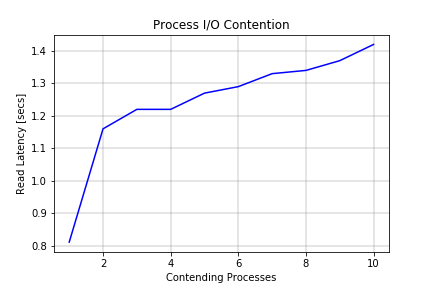
\includegraphics[scale=0.6]{images/process_contention.png}
\label{processcontention}
\end{figure}

\subsubsection{Discussion}
As expected, we find a correlation between the number of contending processes and the average latency they experience in issuing random disk I/O requests. We expect the hardware overhead to increase as the number of contending processors increases. We also expect that the majority of the time spent here will be in waiting for disk accesses as blocks are requested. When a file requests a block, it will be blocked waiting for disk. This forces a context switch to another process, which is also blocking on disk access. This causes a significant amount of disk contention on the hardware level.

We are confident that our measurements take into account all aspects of our goal. We had some difficulty with library implementations and some of the measurements have some interesting properties, like the sharp increase past one process, however we tried many different implementations including forking, sequential file access, random file access, block access, and others. We have reported our most consistent results.

%%%%%%%%%%%%%%%%%%%%%%%%%%%%%%%%%%%%%%
% Conclusion
%%%%%%%%%%%%%%%%%%%%%%%%%%%%%%%%%%%%%%
\section{Conclusion}
Benchmarking modern operating systems requires a nuanced, and deep command of a myriad of optimizations happening during program run-time including optimization semantics of C libraries, Kernel mechanisms and hardware components.  We designed each experiment to isolate and mitigate against these optimizations, in order to hone in on specific functionality we are interested in profiling. To the best of our abilities, each experiment is orchestrated to preserve system integrity, and repeated for statistical convergence and we  feel confident that our results reflect realistic performance metrics for our system setup.

A key takeaway for us is that a deep understanding of system implementation is crucial to careful experiment design. Often, such specifications are not readily available, and both external research and clever experimentation is required to understand what optimizations are happening under the hood. In total, this project lent itself to our growth both as systems engineers, and  experiment designers and has colored our understanding of the trade-off space in OS design, and the measuring tools required to understand those trade-offs.

%%%%%%%%%%%%%%%%%%%%%%%%%%%%%%%%%%%%%%
% Acknowledgments
%%%%%%%%%%%%%%%%%%%%%%%%%%%%%%%%%%%%%%
\begin{acks}
We would like to thank Professor Yuanyuan Zhou for her patience and direction throughout the term. We would also like to thank the TAs Gustavo Umbelino and Chengcheng Xiang for answering our questions and providing timely and helpful feedback on this paper as it progressed.  
\end{acks}
%%%%%%%%%%%%%%%%%%%%%%%%%%%%%%%%%%%%%%

\bibliographystyle{ACM-Reference-Format}
\bibliography{bibliography}

\end{document}
